\documentclass[border=6pt]{standalone}
\usepackage{amsmath}
\usepackage{tikz}
\usetikzlibrary{shapes.geometric,arrows.meta,positioning,fit,backgrounds,calc}
\begin{document}
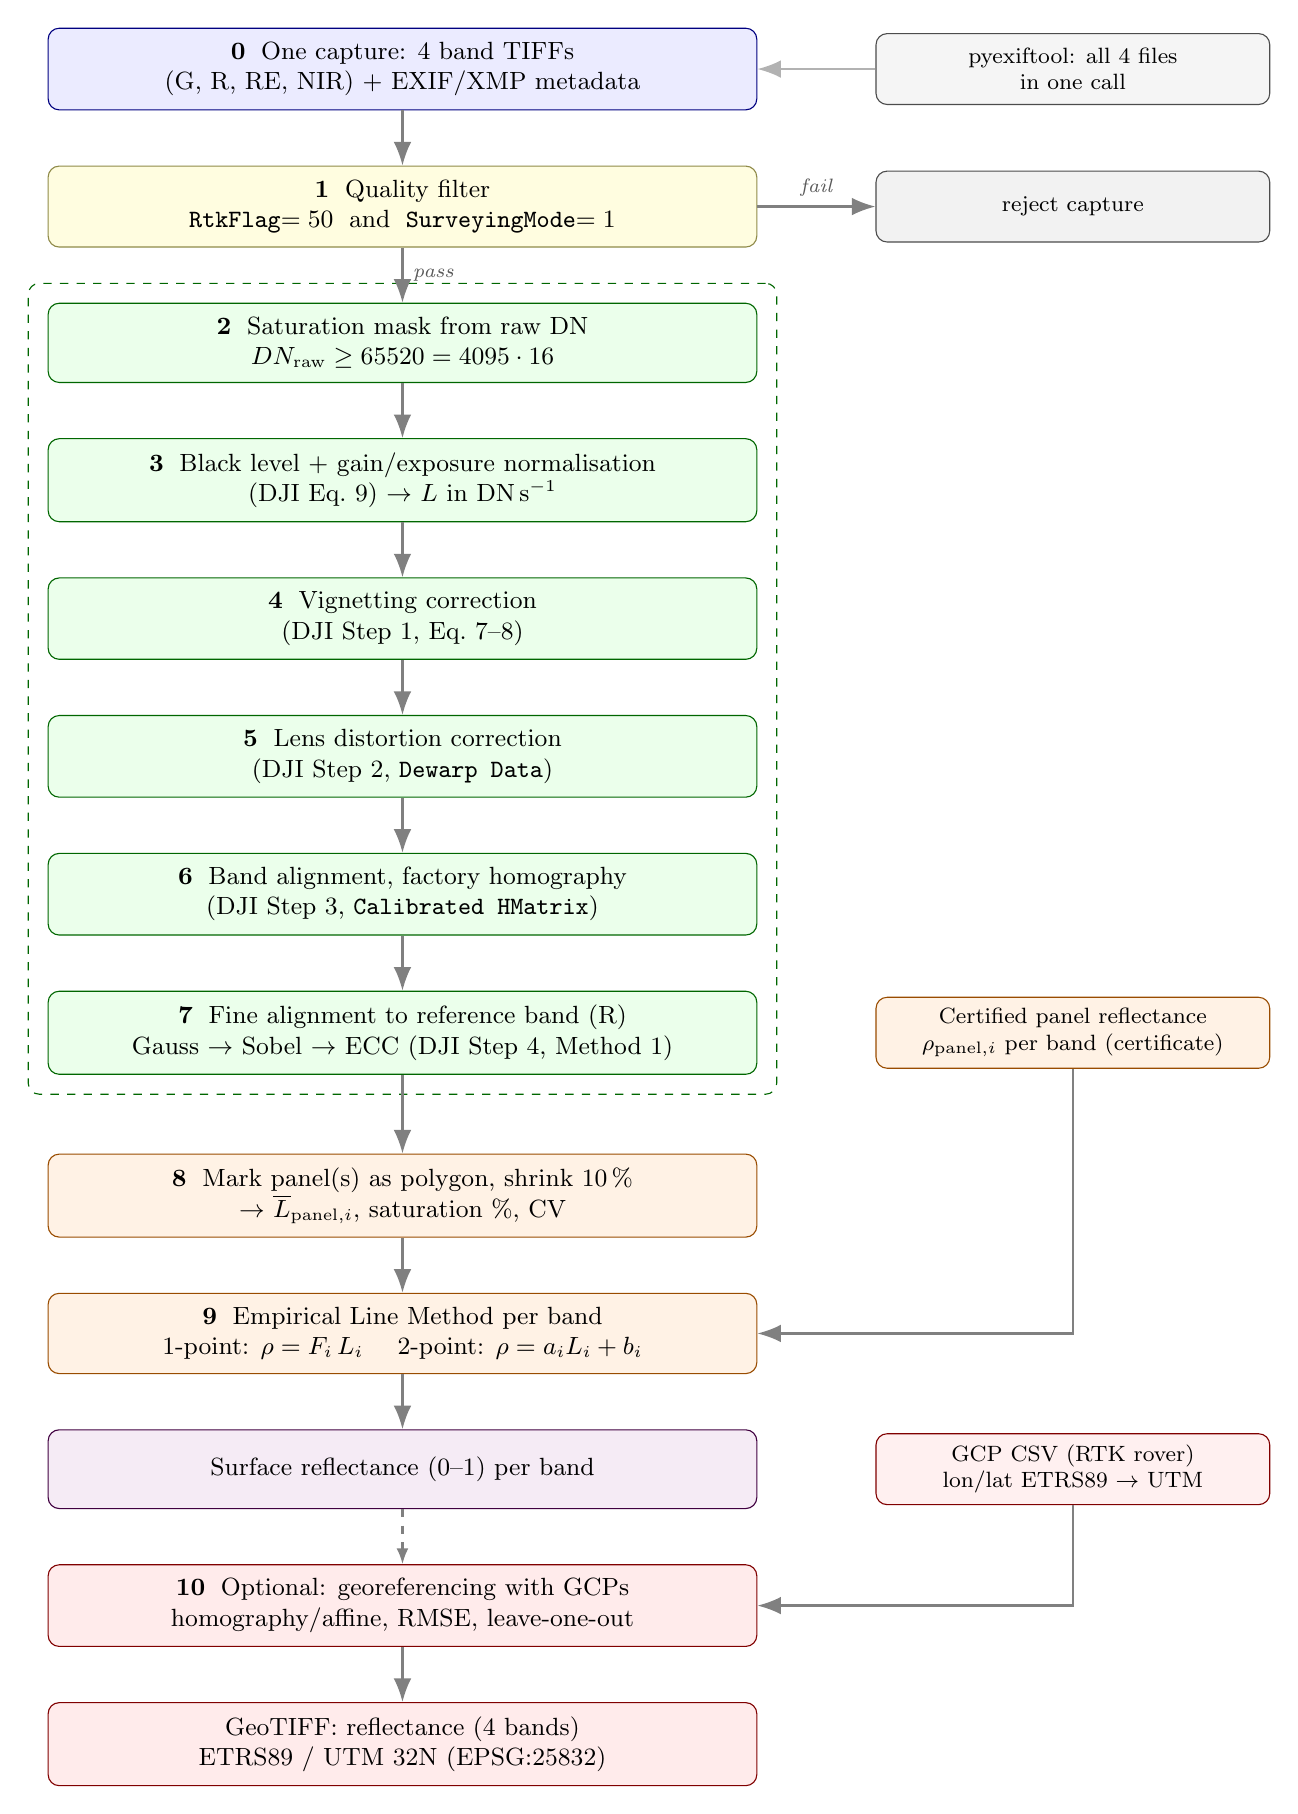
\begin{tikzpicture}[
  node distance=7mm and 8mm,
  box/.style={draw, rounded corners, align=center, minimum width=9.0cm, minimum height=1.0cm, font=\small, inner sep=5pt},
  small/.style={draw, rounded corners, align=center, minimum width=5.0cm, minimum height=0.9cm, font=\footnotesize, inner sep=4pt},
  arr/.style={-{Latex[length=3mm]}, thick, gray},
  darr/.style={-{Latex[length=2mm]}, thick, gray, dashed},
  lab/.style={font=\scriptsize\itshape, text=gray!70!black}
]
% --- input
\node[box, fill=blue!8, draw=blue!50!black] (raw) {\textbf{0}\; One capture: 4 band TIFFs\\(G, R, RE, NIR) + EXIF/XMP metadata};
\node[small, fill=gray!8, draw=gray!60!black, right=15mm of raw] (meta) {pyexiftool: all 4 files\\in one call};
% --- quality
\node[box, fill=yellow!12, draw=yellow!50!black, below=of raw] (qual) {\textbf{1}\; Quality filter\\\texttt{RtkFlag}$=50$ \;and\; \texttt{SurveyingMode}$=1$};
\node[small, fill=gray!10, draw=gray!60!black, right=15mm of qual] (reject) {reject capture};
% --- per band
\node[box, fill=green!8, draw=green!40!black, below=of qual] (sat) {\textbf{2}\; Saturation mask from raw DN\\$DN_{\text{raw}} \geq 65520 = 4095\cdot 16$};
\node[box, fill=green!8, draw=green!40!black, below=of sat] (norm) {\textbf{3}\; Black level + gain/exposure normalisation\\(DJI Eq.~9) $\to$ $L$ in DN\,s$^{-1}$};
\node[box, fill=green!8, draw=green!40!black, below=of norm] (vig) {\textbf{4}\; Vignetting correction\\(DJI Step~1, Eq.~7--8)};
\node[box, fill=green!8, draw=green!40!black, below=of vig] (dist) {\textbf{5}\; Lens distortion correction\\(DJI Step~2, \texttt{Dewarp Data})};
\node[box, fill=green!8, draw=green!40!black, below=of dist] (hom) {\textbf{6}\; Band alignment, factory homography\\(DJI Step~3, \texttt{Calibrated HMatrix})};
\node[box, fill=green!8, draw=green!40!black, below=of hom] (ecc) {\textbf{7}\; Fine alignment to reference band (R)\\Gauss $\to$ Sobel $\to$ ECC (DJI Step~4, Method~1)};
% background for per-band block
\begin{scope}[on background layer]
  \node[draw=green!40!black, dashed, rounded corners, fit=(sat)(ecc), inner sep=7pt] (perband) {};
\end{scope}
% --- panels
\node[small, fill=orange!10, draw=orange!60!black, right=15mm of ecc] (cert) {Certified panel reflectance\\$\rho_{\text{panel},i}$ per band (certificate)};
\node[box, fill=orange!10, draw=orange!60!black, below=10mm of ecc] (panel) {\textbf{8}\; Mark panel(s) as polygon, shrink 10\,\%\\$\to$ $\overline{L}_{\text{panel},i}$, saturation \%, CV};
\node[box, fill=orange!10, draw=orange!60!black, below=of panel] (elm) {\textbf{9}\; Empirical Line Method per band\\1-point: $\rho = F_i\,L_i$ \quad 2-point: $\rho = a_i L_i + b_i$};
\node[box, fill=violet!8, draw=violet!50!black, below=of elm] (refl) {Surface reflectance (0--1) per band};
% --- georef
\node[small, fill=red!6, draw=red!50!black, right=15mm of refl] (gcpcsv) {GCP CSV (RTK rover)\\lon/lat ETRS89 $\to$ UTM};
\node[box, fill=red!8, draw=red!50!black, below=of refl] (geo) {\textbf{10}\; Optional: georeferencing with GCPs\\homography/affine, RMSE, leave-one-out};
\node[box, fill=red!8, draw=red!50!black, below=of geo] (final) {GeoTIFF: reflectance (4 bands)\\ETRS89 / UTM 32N (EPSG:25832)};
% --- arrows
\draw[arr] (raw) -- (qual);
\draw[arr, gray!60] (meta) -- (raw);
\draw[arr] (qual) -- node[lab, above]{fail} (reject);
\draw[arr] (qual) -- node[lab, right]{pass} (sat);
\draw[arr] (sat) -- (norm);
\draw[arr] (norm) -- (vig);
\draw[arr] (vig) -- (dist);
\draw[arr] (dist) -- (hom);
\draw[arr] (hom) -- (ecc);
\draw[arr] (ecc) -- (panel);
\draw[arr] (panel) -- (elm);
\draw[arr] (cert) |- (elm.east);
\draw[arr] (elm) -- (refl);
\draw[darr] (refl) -- (geo);
\draw[arr] (gcpcsv) |- (geo.east);
\draw[arr] (geo) -- (final);
\end{tikzpicture}
\end{document}
